% =====================================================================
%  YUYOS DE LA QUEBRADA DE CAFAYATE
%  Libro ilustrado — Centro Experimental de Formación Agroecológica
%
%  Compilar con:   pdflatex cafayate.tex   (dos veces, por el índice)
%  o bien:         latexmk -pdf cafayate.tex
%
%  Las ilustraciones definitivas van en la carpeta ./img con los nombres
%  que se usan en este archivo (01-cubierta.jpg ... 23-contratapa.jpg).
%  Si se reemplaza alguna, mantener el mismo nombre y la misma proporción
%  para que el libro compile sin tocar una sola línea.
% =====================================================================

\documentclass[11pt,twoside,openright]{book}

% ------------------------- Idioma y tipografía -----------------------
\usepackage[utf8]{inputenc}
\usepackage[T1]{fontenc}
\usepackage[spanish,es-noshorthands,es-tabla]{babel}
\usepackage{mathpazo}                 % texto: Palatino
\renewcommand{\sfdefault}{pag}        % títulos: Avant Garde Gothic
\usepackage{microtype}
\usepackage{textcomp}

% Si querés una tipografía aún más fina y tenés XeLaTeX + EB Garamond:
%   comentá las tres líneas de mathpazo/sfdefault y usá
%   \usepackage{fontspec}
%   \setmainfont{EB Garamond}
%   \setsansfont{Alegreya Sans}

% ------------------------------ Paquetes -----------------------------
\usepackage{graphicx}
\usepackage{array}
\newcolumntype{L}[1]{>{\raggedright\arraybackslash}p{#1}}
\usepackage{xcolor}
\usepackage[a4paper]{geometry}
\usepackage{titlesec}
\usepackage{fancyhdr}
\usepackage{enumitem}
\usepackage{lettrine}
\usepackage{multicol}
\usepackage{eso-pic}
\usepackage{tikz}
\usetikzlibrary{fadings}
\usepackage[skins,breakable]{tcolorbox}
\usepackage{pgfornament}
\usepackage[hidelinks]{hyperref}
\urlstyle{same}

% ---------------------------- Formato de página ----------------------
% Libro de 17 x 24 cm, proporción clásica de libro ilustrado.
\geometry{
  paperwidth=17cm, paperheight=24cm,
  inner=2.3cm, outer=1.9cm, top=2.4cm, bottom=2.6cm,
  headsep=1.1em, footskip=1.4cm
}

% ------------------------------- Paleta ------------------------------
\definecolor{verdehuerta}{HTML}{3F4A2E}
\definecolor{verdehoja}  {HTML}{7C8A5A}
\definecolor{terracota}  {HTML}{9C3F22}
\definecolor{ocre}       {HTML}{C28A34}
\definecolor{crema}      {HTML}{FBF4E6}
\definecolor{tinta}      {HTML}{2B2B28}
\definecolor{gris}       {HTML}{7A7A72}

\color{tinta}

% --------------------------- Títulos de parte ------------------------
\titleformat{\part}[display]
  {\sffamily\bfseries\color{verdehuerta}\filcenter}
  {\normalsize\normalfont\color{terracota}\MakeUppercase{\partname~\thepart}}
  {1.2em}{\Huge}
\titlespacing*{\part}{0pt}{2em}{2em}

% -------------------------- Títulos de capítulo ----------------------
\titleformat{\chapter}[display]
  {\sffamily\color{verdehuerta}}
  {\raggedright\normalfont\normalsize\color{terracota}%
     \rule[0.35em]{1.6cm}{0.6pt}\hspace{0.6em}%
     \MakeUppercase{\chaptername~\thechapter}}
  {0.9em}
  {\raggedright\bfseries\LARGE}
  [\vspace{0.6em}{\color{verdehoja}\rule{\textwidth}{1.2pt}}]
\titlespacing*{\chapter}{0pt}{-1.2em}{2.2em}

\titleformat{\section}
  {\sffamily\bfseries\large\color{verdehuerta}}{}{0pt}{}
\titlespacing*{\section}{0pt}{1.6em}{0.5em}

\titleformat{\subsection}
  {\sffamily\bfseries\normalsize\color{terracota}}{}{0pt}{}
\titlespacing*{\subsection}{0pt}{1.2em}{0.3em}

% ------------------------------ Encabezados --------------------------
\pagestyle{fancy}
\fancyhf{}
\renewcommand{\headrulewidth}{0pt}
\renewcommand{\footrulewidth}{0pt}
\fancyhead[LE]{\sffamily\scriptsize\color{gris}\MakeUppercase{Yuyos de la Quebrada}}
\fancyhead[RO]{\sffamily\scriptsize\color{gris}\nouppercase{\leftmark}}
\fancyfoot[LE,RO]{\sffamily\small\color{verdehuerta}\thepage}
\renewcommand{\chaptermark}[1]{\markboth{#1}{}}

\fancypagestyle{plain}{\fancyhf{}%
  \fancyfoot[LE,RO]{\sffamily\small\color{verdehuerta}\thepage}%
  \renewcommand{\headrulewidth}{0pt}}

% Comportamiento de las figuras flotantes
\setcounter{topnumber}{2}\setcounter{bottomnumber}{1}\setcounter{totalnumber}{3}
\renewcommand{\topfraction}{0.92}
\renewcommand{\bottomfraction}{0.75}
\renewcommand{\textfraction}{0.06}
\renewcommand{\floatpagefraction}{0.75}

% Las páginas en blanco de cortesía van limpias, sin encabezado ni folio
\makeatletter
\def\cleardoublepage{\clearpage\if@twoside\ifodd\c@page\else
  \hbox{}\thispagestyle{empty}\newpage\if@twocolumn\hbox{}\newpage\fi\fi\fi}
\makeatother

% Interlineado y párrafos
\linespread{1.08}
\setlength{\parindent}{1.2em}
\setlength{\emergencystretch}{2em}

% ---------------------------- Cajas de texto -------------------------
% Transcripción del cuaderno original
\newtcolorbox{cuaderno}[1][Del cuadernillo original]{
  enhanced, breakable,
  colback=crema, colframe=ocre,
  boxrule=0pt, leftrule=2.5pt,
  arc=0pt, outer arc=0pt,
  left=1.1em, right=1.1em, top=0.9em, bottom=0.9em,
  fontupper=\itshape\small,
  title={\sffamily\bfseries\scriptsize\color{terracota}\MakeUppercase{#1}},
  attach title to upper={\par\vspace{0.5em}},
  coltitle=terracota
}

% Receta o procedimiento paso a paso
\newtcolorbox{practica}[1]{
  enhanced, breakable,
  colback=white, colframe=verdehoja,
  boxrule=0.8pt, arc=2pt,
  left=1.1em, right=1.1em, top=0.9em, bottom=0.9em,
  fonttitle=\sffamily\bfseries\small,
  coltitle=white, colbacktitle=verdehoja,
  title={#1}
}

% Advertencia / precaución
\newtcolorbox{cuidado}[1][Atención]{
  enhanced, breakable,
  colback=white, colframe=terracota,
  boxrule=0.8pt, arc=0pt,
  left=1.1em, right=1.1em, top=0.8em, bottom=0.8em,
  fontupper=\small,
  fonttitle=\sffamily\bfseries\scriptsize,
  coltitle=white, colbacktitle=terracota,
  title={\MakeUppercase{#1}}
}

% --------------------------- Fichas de herbario ----------------------
% \begin{planta}{Nombre común}{Nombre científico}{Parte que se usa}
\newenvironment{planta}[3]{%
  \par\vspace{1.4em}\noindent
  {\sffamily\bfseries\large\color{verdehuerta}#1}\quad
  {\itshape\small\color{gris}#2}\par
  \vspace{0.15em}
  \noindent{\color{verdehoja}\rule{\textwidth}{0.6pt}}\par
  \vspace{0.25em}
  \noindent{\sffamily\scriptsize\color{terracota}\MakeUppercase{Se usa: }#3}\par
  \vspace{0.55em}\small\ignorespaces
}{\par\vspace{0.4em}}

% ------------------------------- Utilidades --------------------------
% Imagen a caja completa con epígrafe
\newcommand{\lamina}[3][\textwidth]{%
  \begin{figure}[htbp]\centering
    \includegraphics[width=#1]{#2}\par\vspace{0.5em}
    {\footnotesize\sffamily\color{gris}#3}
  \end{figure}}

% Imagen a página entera (sin encabezado)
% La altura se limita para que imagen + epígrafe quepan siempre en una
% sola página: si desbordan, LaTeX deja una página vacía antes de la
% lámina y el encabezado reaparece sobre la ilustración.
\newcommand{\laminapagina}[2]{%
  \clearpage
  \thispagestyle{empty}
  \vspace*{\fill}
  \begin{center}
    \includegraphics[width=\textwidth,height=0.84\textheight,keepaspectratio]{#1}\par\vspace{0.7em}
    {\footnotesize\sffamily\color{gris}#2}
  \end{center}
  \vspace*{\fill}\clearpage}

% Parte con lámina: la página de la parte va en impar y la ilustración
% ocupa el verso siguiente (en lugar de la página en blanco automática).
\makeatletter
\newcommand{\parteconlamina}[3]{%
  \cleardoublepage
  \@openrightfalse
  \part{#1}%
  \@openrighttrue
  \laminapagina{#2}{#3}}

% Salto a página par (verso): para la contratapa, que debe ser la última
% cara del libro.
\newcommand{\clearalapar}{%
  \clearpage
  \ifodd\c@page\hbox{}\thispagestyle{empty}\newpage\fi}
\makeatother

% Entrada del índice de plantas: nombre, puntos, página y científico
\newcommand{\entradaplanta}[3]{%
  \par\noindent{\sffamily\bfseries\footnotesize\color{verdehuerta}#1}%
  \nobreak\dotfill\nobreak{\sffamily\footnotesize\pageref{#2}}\par
  \nobreak\noindent\hspace*{0.8em}#3\par\vspace{0.35em}}

% Filete ornamental de cierre de capítulo
\newcommand{\cierre}{%
  \par\vspace{1.6em}
  \begin{center}\color{verdehoja}\pgfornament[width=2.6cm]{88}\end{center}
  \vspace{0.4em}}

% Epígrafe bajo el título de capítulo
\newcommand{\epigrafe}[2]{%
  \begin{flushright}\begin{minipage}{0.78\textwidth}
    \raggedleft\itshape\small\color{gris}#1\par
    \vspace{0.2em}{\sffamily\scriptsize\upshape\color{terracota}#2}
  \end{minipage}\end{flushright}\vspace{1.4em}}

% Capitular
\newcommand{\capitular}[2]{%
  \lettrine[lines=3, findent=0.2em, nindent=0em,
            slope=0em, lhang=0.1]
  {\color{terracota}\sffamily\bfseries #1}{\scshape #2}}

% Lista de pasos numerados
\newcommand{\numeropaso}[1]{%
  \begin{tikzpicture}[baseline=(n.base)]
    \node[circle, fill=verdehoja, text=white, inner sep=1.7pt,
          font=\sffamily\bfseries\scriptsize] (n) {#1};
  \end{tikzpicture}}
\newlist{pasos}{enumerate}{1}
\setlist[pasos]{label=\protect\numeropaso{\arabic*},
  leftmargin=2.2em, itemsep=0.45em, topsep=0.5em}

\setlist[itemize]{label=\textcolor{verdehoja}{\textbullet},
  leftmargin=1.5em, itemsep=0.3em, topsep=0.4em}

% =====================================================================
\hypersetup{
  pdftitle={Yuyos de la Quebrada de Cafayate},
  pdfauthor={María Eugenia Orellana},
  pdfsubject={Plantas medicinales del monte quebradeño},
  pdfkeywords={yuyos, plantas medicinales, Cafayate, Valles Calchaquíes, fitoterapia}}

\begin{document}
\frenchspacing

% La cubierta se numera aparte para que sus anclas no choquen con las
% páginas 1 y 2 del cuerpo del libro (avisos «destination with the same
% identifier» de hyperref).
\pagenumbering{Alph}

% =====================================================================
%  CUBIERTA
% =====================================================================
\begin{titlepage}
\thispagestyle{empty}
\AddToShipoutPictureBG*{%
  \put(0,0){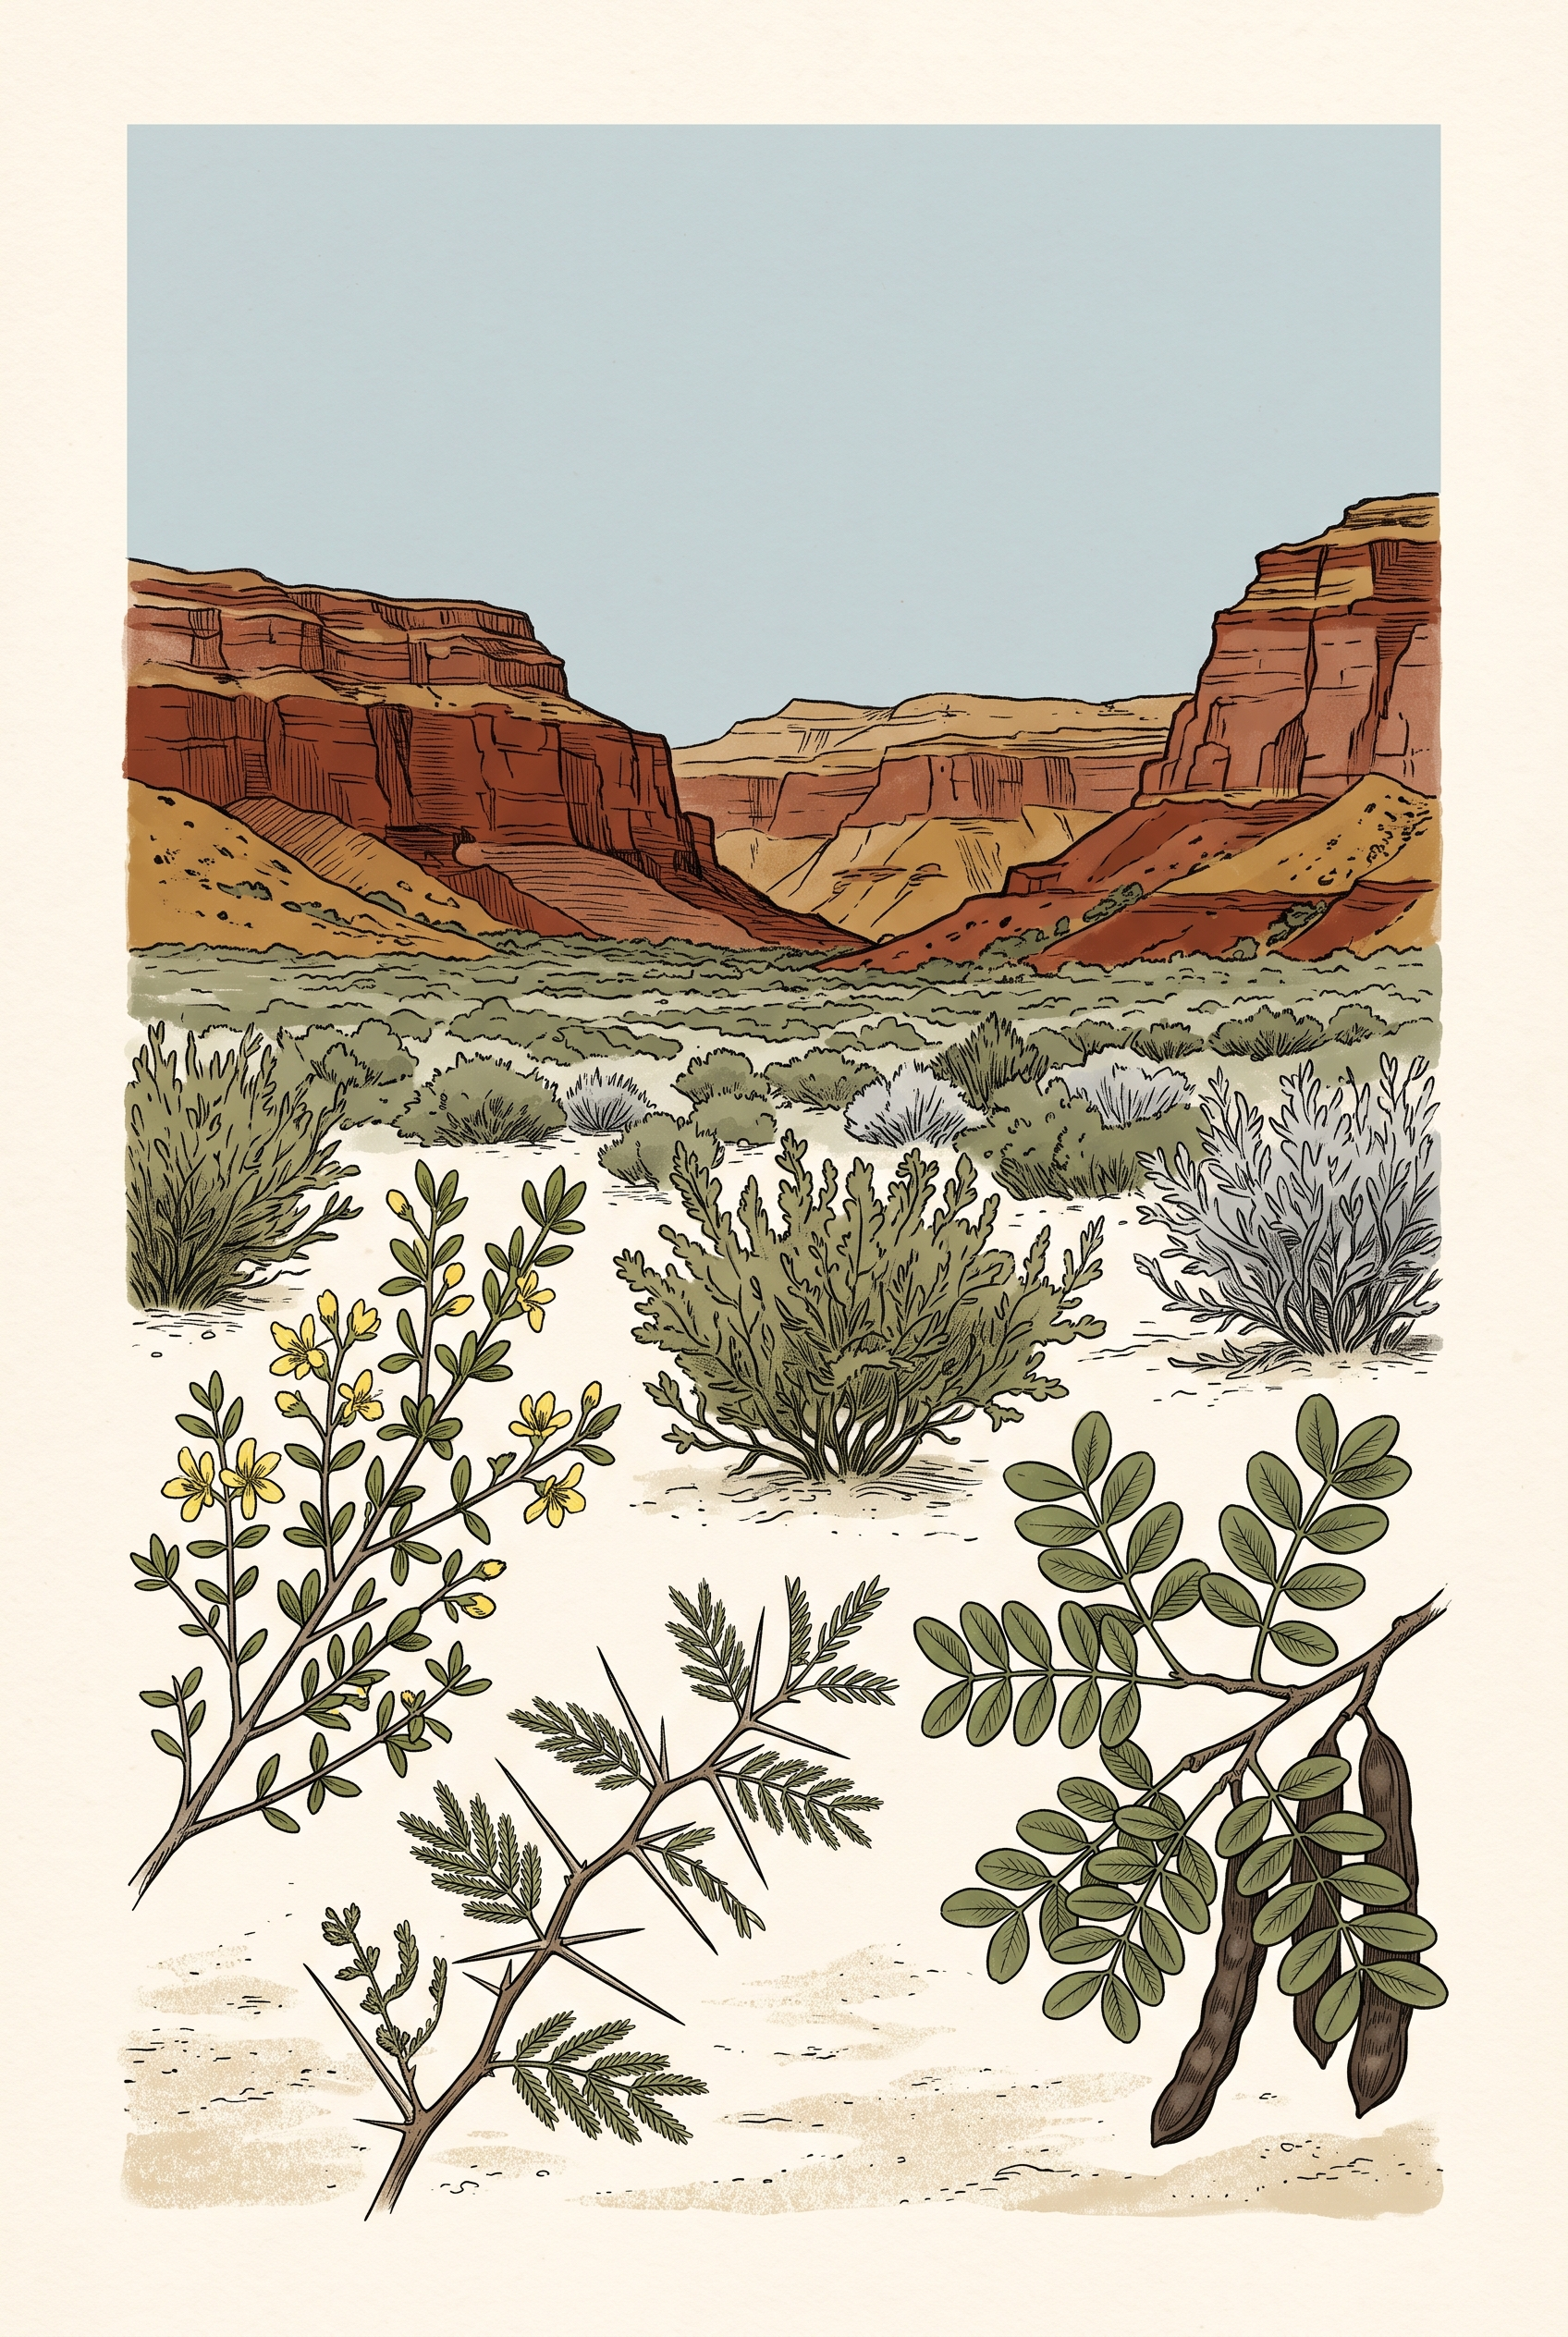
\includegraphics[width=\paperwidth,height=\paperheight]{img/01-cubierta.jpg}}}
\begin{tikzpicture}[remember picture, overlay]
  \fill[verdehuerta, opacity=0.74, path fading=south]
        (current page.north west) rectangle
        ([yshift=-10.6cm]current page.north east);
  \fill[verdehuerta, opacity=0.85, path fading=north]
        (current page.south west) rectangle
        ([yshift=4.6cm]current page.south east);
  \node[anchor=north, inner sep=0pt] at ([yshift=-2.0cm]current page.north)
    {\begin{minipage}{0.82\paperwidth}
       \centering
       {\sffamily\bfseries\fontsize{27}{31}\selectfont\color{crema} Yuyos}\\[0.25em]
       {\sffamily\fontsize{15}{19}\selectfont\color{crema} de la Quebrada de Cafayate}\\[0.6em]
       {\color{ocre}\rule{5cm}{1pt}}\\[0.7em]
       {\sffamily\fontsize{11}{14}\selectfont\color{crema}
        MARÍA EUGENIA ORELLANA}
     \end{minipage}};
  \node[anchor=south, inner sep=0pt] at ([yshift=1.5cm]current page.south)
    {\begin{minipage}{0.82\paperwidth}
       \centering
       {\sffamily\fontsize{8.5}{11}\selectfont\color{crema}
        LA BOTICA COMPLETA, A UN KILÓMETRO A LA REDONDA\\[0.3em]
        VALLES CALCHAQUÍES · SALTA}
     \end{minipage}};
\end{tikzpicture}
\end{titlepage}

\frontmatter
\pagestyle{empty}

% --- Portadilla ---
\cleardoublepage
\null\vspace*{6cm}
\begin{center}
  {\sffamily\fontsize{20}{24}\selectfont\color{verdehuerta} Yuyos de la Quebrada}\\[0.6em]
  {\color{verdehoja}\pgfornament[width=2.2cm]{88}}
\end{center}
\clearpage

% --- Portada ---
\cleardoublepage
\null\vspace*{3.2cm}
\begin{center}
  {\sffamily\fontsize{26}{30}\selectfont\color{verdehuerta} Yuyos}\\[0.5em]
  {\sffamily\fontsize{15}{19}\selectfont\color{verdehuerta} de la Quebrada de Cafayate}\\[0.9em]
  {\color{terracota}\rule{6cm}{1pt}}\\[1.2em]
  {\itshape\large\color{gris} Las plantas que curan en el monte quebradeño}\\[2.2cm]
  {\sffamily\fontsize{14}{18}\selectfont\color{terracota} MARÍA EUGENIA ORELLANA}\\[2.6cm]
  {\sffamily\small\color{verdehuerta} VALLES CALCHAQUÍES · SALTA}\\[2.2cm]
  {\color{verdehoja}\pgfornament[width=3cm]{71}}
\end{center}
\clearpage

% --- Créditos (verso de la portada) ---
\null\vfill
\noindent{\footnotesize\setlength{\parindent}{0pt}
\textsf{\textbf{Yuyos de la Quebrada de Cafayate}}\par
\vspace{0.5em}
Edición ilustrada. Edición de autor, \the\year.\par
\vspace{0.9em}
\copyright{} María Eugenia Orellana.\par
\vspace{0.9em}
Texto e investigación de campo: María Eugenia Orellana, a partir de su
cuadernillo original y de las conversaciones con los vecinos de la
Quebrada de Cafayate.\par
\vspace{0.9em}
Ilustraciones: Eduardo Diedrich.\par
Diseño y composición tipográfica: Eduardo Diedrich.\par
\vspace{0.9em}
Se permite y se agradece la reproducción total o parcial de esta obra
con fines educativos y comunitarios, citando la fuente. El monte, como
el conocimiento, se cuida compartiéndolo.\par
\vspace{0.9em}
Impreso en Argentina.\par
}
\vspace{2em}
\clearpage

% --- Dedicatoria ---
\cleardoublepage
\null\vspace*{7cm}
\begin{flushright}
  \begin{minipage}{0.68\textwidth}
    \raggedleft\itshape\color{verdehuerta}
    Para mi hermanito del alma.
  \end{minipage}
\end{flushright}
\clearpage

% --- Nota de lectura ---
\cleardoublepage
\null\vspace*{3.4cm}
\begin{center}
  {\sffamily\bfseries\color{verdehuerta} NOTA DE LECTURA}\\[0.4em]
  {\color{verdehoja}\rule{4cm}{0.8pt}}
\end{center}
\vspace{1.2em}
\noindent\small
Este libro registra un saber vivo: el uso que la gente de los Valles
Calchaquíes le da a las plantas que crecen a su alrededor. Ese saber es
\textbf{patrimonio cultural} y merece ser conservado con precisión, tal
como fue transmitido.

\vspace{0.7em}
\noindent\small
No es, en cambio, un manual de tratamiento. Las atribuciones que
aparecen en cada ficha son las que la tradición le da a cada planta; no
constituyen indicaciones médicas, no reemplazan el diagnóstico ni el
tratamiento profesional, y no deben usarse para postergar una consulta.
Donde la tradición atribuye a una planta la capacidad de tratar
enfermedades graves —cáncer, tuberculosis, infecciones severas— el libro
lo dice con todas las letras: \textbf{no existe evidencia clínica que lo
respalde}, y abandonar un tratamiento médico por una infusión es
peligroso.

\vspace{0.7em}
\noindent\small
Varias de estas plantas son activas de verdad, y por eso mismo pueden
ser tóxicas, abortivas o interactuar con medicamentos. Dos de ellas
—el chamico y el palán palán— son directamente venenosas y figuran acá
únicamente para que se las sepa reconocer y evitar. Otras tres —la
retama, la cepa caballo y el paico— tienen toxicidad conocida y llevan
su advertencia en la ficha. Por esa razón este libro no incluye dosis
para ninguna planta tóxica o psicoactiva, aunque el cuadernillo original
las traiga.

\vspace{0.7em}
\noindent\small
En embarazo, lactancia, infancia, enfermedades crónicas o junto con
medicación, cualquier planta debe consultarse con un profesional de la
salud.

\vspace{0.7em}
\noindent\small
\textbf{Ante una sospecha de intoxicación}, llamar sin demora al Centro
Nacional de Intoxicaciones (Hospital Posadas), \textbf{0800-333-0160}, o
acudir a la guardia más cercana llevando una muestra de la planta.
\clearpage

% --- Índice ---
\cleardoublepage
\pagestyle{fancy}
\renewcommand{\contentsname}{Índice}
% Una línea más de caja en la página del índice: sin esto, la última
% entrada («Colofón») queda sola en una página nueva.
\addtocontents{toc}{\protect\enlargethispage{3\baselineskip}}
\tableofcontents
\cleardoublepage

% --- Introducción ---
\chapter*{Palabras de la autora}
\addcontentsline{toc}{chapter}{Palabras de la autora}
\markboth{Palabras de la autora}{}

\capitular{E}{sta investigación} parte de una necesidad personal: la de
identificar las plantas con las que nos estábamos curando mi hija y yo,
desde que llegamos a vivir a la Quebrada de Cafayate. Preguntando a uno
y a otro, llegué a darme cuenta de que teníamos alrededor la botica
completa.

Existe una idea antigua que dice que en un perímetro de un kilómetro a
la redonda tenemos todo lo que necesitamos para sanarnos —suponiendo,
claro, que ese entorno sea natural. Por eso considero al ser urbano
huérfano de madre naturaleza.

Este sistema nos fue alejando cada vez más de la sabiduría antigua y de
la intuición innata que todos llevamos dentro para sanar nuestro cuerpo
y nuestra alma, que al final son una sola entidad indivisible. Al tener
un enfermo más, tienen un eslabón más en la larga cadena de consumo.
Estamos alimentando al monstruo sin siquiera notarlo.

De las plantas medicinales, que son casi todas, porque cualquiera tiene
algún principio activo, cuatro de cada cinco son de recolección
silvestre. Si no le ponemos freno a esta depredación sin límites,
nuestra madre va a tener que cerrar la botica.

\vspace{1.6em}
\begin{flushright}
  {\itshape\color{verdehuerta} Pachamama Munaskka Munata}\\[0.2em]
  {\sffamily\footnotesize\color{gris} MADRE TIERRA AMADA}
\end{flushright}
\vspace{1em}
\begin{flushright}
  {\sffamily\small\color{verdehuerta} MARÍA EUGENIA ORELLANA}\\[0.2em]
  {\sffamily\footnotesize\color{gris} QUEBRADA DE CAFAYATE}
\end{flushright}
\cierre

\laminapagina{img/02-frontispicio.jpg}{%
  «La enfermedad es un desencuentro entre nuestros cuerpos y nuestras
  almas. Aparece cuando nos volvemos sordos a la voz interior.»
  \\ Edward Bach}

% =====================================================================
\mainmatter
\parteconlamina{La botica a un kilómetro a la redonda}
  {img/03-parte1-apertura.jpg}{%
  La Quebrada de Cafayate al amanecer. Entre los cerros colorados y el
  cauce seco crece una farmacia entera.}

% ---------------------------------------------------------------------
\chapter{El monte como botica}
\epigrafe{Teníamos a nuestro alrededor\\ la botica completa.}{CUADERNILLO ORIGINAL}

\capitular{L}{a quebrada} no parece, a primera vista, un lugar generoso.
Suelo arenoso, poca lluvia, sol duro, amplitud térmica brutal entre el
mediodía y la madrugada. Y sin embargo, justamente por eso, muchas de
las plantas que crecen acá son muy activas: una planta que vive bajo
estrés suele producir más resinas, más aceites esenciales, más
alcaloides. Esos
compuestos son su defensa, y son también lo que buscamos cuando la
usamos.

\lamina[0.85\textwidth]{img/04-botica-kilometro.jpg}{%
  El kilómetro a la redonda: la idea que organiza este libro. Lo que
  crece cerca es lo que está adaptado al clima, la altura y la humedad
  del lugar donde vivimos.}

\section{Por qué lo cercano}

La idea del kilómetro a la redonda no es sólo una metáfora romántica.
Las plantas que prosperan en un sitio son las que el clima, la altura y
la humedad seleccionaron ahí, y son las que la gente del lugar tuvo
siempre a mano para probar, observar y recordar. La tradición agrega una
idea más, que conviene leer como tal: que el entorno ofrece remedio para
los males que él mismo produce —donde el aire es seco y la altura
castiga, las respiratorias; donde el agua es dura, las que trabajan
sobre el riñón—.

Además, lo cercano se conoce. Uno sabe dónde está esa mata de jarilla,
en qué mes florece el chañar, qué año dio más algarroba. Ese conocimiento
acumulado vale más que cualquier etiqueta.

\section{Recolectar sin depredar}

Se estima que cuatro de cada cinco plantas medicinales que se consumen
en el país son de recolección silvestre. Eso significa que cada manojo que sacamos sale
de una población real, que tarda en reponerse. La regla en la quebrada
es simple y no se negocia.

\begin{practica}{Reglas de recolección}
\begin{pasos}
  \item Nunca más de un tercio de una misma planta, y nunca todas las
  plantas de un mismo sitio.
  \item No arrancar de raíz salvo que la raíz sea lo que se usa, y en
  ese caso dejar en pie a las vecinas.
  \item Cosechar a la mañana, después de que se evaporó el rocío y antes
  del sol fuerte.
  \item Hojas antes de la floración; flores recién abiertas; cortezas y
  raíces a fin de invierno.
  \item Lejos de rutas, de cultivos fumigados y de cursos de agua
  contaminados.
  \item Si una planta escasea en la zona, no se cosecha. Se la deja
  multiplicar y se busca otra que haga lo mismo.
\end{pasos}
\end{practica}

\begin{cuidado}[Identificar antes de usar]
En el monte hay plantas que se parecen entre sí y que no hacen lo mismo:
algunas curan y otras envenenan. Si hay la más mínima duda sobre qué es
lo que se está cosechando, no se usa. Preguntar a alguien que conozca es
parte del método, no una debilidad.
\end{cuidado}

\section{Secado y guardado}

\lamina{img/05-cosecha-secado.jpg}{%
  Manojos secándose a la sombra. El sol directo destruye en dos días los
  aceites esenciales que tardaron una temporada en formarse.}

\begin{itemize}
  \item En manojos chicos, colgados boca abajo, a la sombra y con buena
  ventilación. Nunca al sol ni en horno.
  \item Las hojas están listas cuando se quiebran al doblarlas; las
  flores, cuando pierden humedad pero conservan color.
  \item Guardar en frascos de vidrio, al reparo de la luz, con etiqueta
  de nombre y fecha.
  \item Un año es la vida útil razonable de la mayoría. Pasado ese
  tiempo la planta sigue siendo planta, pero ya no es remedio.
\end{itemize}

\cierre

% ---------------------------------------------------------------------
\chapter{Las preparaciones}
\epigrafe{Los tés medicinales\\ se toman sin endulzar.}{CUADERNILLO ORIGINAL}

\capitular{C}{ada preparación} extrae cosas distintas de la misma planta.
El agua caliente saca lo soluble y lo delicado; el hervor prolongado,
lo que está encerrado en cortezas y raíces; el alcohol, las resinas y
los aceites esenciales; la grasa, lo que debe quedarse en la piel.
Elegir bien la preparación es la mitad del resultado.

\lamina{img/06-preparaciones-infusion.jpg}{%
  Infusión, decocción y cataplasma: tres maneras distintas de pedirle a
  la planta lo que tiene.}

\section{Infusión}

Para hojas y flores. Se calienta el agua hasta antes del hervor, se
vuelca sobre la planta, se tapa —tapar es esencial, ahí se juegan los
aceites esenciales— y se deja reposar entre cinco y diez minutos. La
proporción habitual es de un puñado, unos 20 a 30 gramos, por litro de
agua.

Y una costumbre del cuadernillo que conviene respetar: los tés
medicinales se toman sin endulzar, porque la tradición sostiene que el
azúcar corta las propiedades. Si hace falta endulzar, miel, y poca. Hay
dos excepciones con historia propia: el «quemadillo» con que en el campo
se le quita el amargor al chañar, y los jarabes, que son otra
preparación.

\section{Decocción o cocimiento}

Para cortezas, raíces, tallos leñosos y semillas. La planta se pone en
agua fría, se lleva al hervor y se mantiene tapada entre diez y quince
minutos. Después se deja reposar y se filtra.

\section{Cataplasma y emplasto}

La planta fresca machacada, sola o tibia, aplicada directamente sobre la
piel y sostenida con un paño limpio. Es el formato de las contracturas,
los golpes, los abscesos y las heridas cerradas. Nunca sobre una herida
abierta y sucia sin lavarla antes.

\section{Baños y lavados}

Una decocción concentrada, colada y volcada en el agua del baño o del
lavatorio. Es la vía de los dolores reumáticos, de los pies fríos y de
las afecciones de la piel: la planta trabaja sin pasar por el estómago.

\section{Tintura madre}

\begin{cuaderno}
Preparación de una maceración a base de alcohol, que extrae las
propiedades de la planta. De la tintura madre se derivan las microdosis
y la bebida plus.
\end{cuaderno}

\begin{practica}{Tintura madre}
\begin{pasos}
  \item Llenar un frasco de vidrio con la planta: hasta la mitad si está
  seca, hasta arriba si está fresca y picada.
  \item Cubrir completamente con alcohol apto para consumo, rebajado con
  agua hasta unos 40 a 70 grados según la planta. Lo que toca el aire se
  enmohece.
  \item Cerrar, etiquetar con nombre y fecha, guardar en oscuridad.
  \item Agitar todos los días durante tres o cuatro semanas.
  \item Colar con lienzo, exprimir bien y envasar en frasco oscuro con
  gotero.
\end{pasos}
\end{practica}

\lamina{img/07-tintura-madre.jpg}{%
  Maceración en curso y tinturas ya coladas, en frascos ámbar
  etiquetados con nombre y fecha.}

\section{Posología tradicional}

Las pautas que siguen son las que figuran en el cuadernillo original,
para plantas de uso corriente y no tóxicas. No se aplican a ninguna de
las plantas señaladas con advertencia en este libro, ni reemplazan la
indicación de un profesional.

\begin{description}[leftmargin=0pt, style=nextline, font=\sffamily\bfseries\color{verdehuerta}]
  \item[Tintura madre.] El primer día es de impregnación: una gota cada
  hora. Los días siguientes, 20 gotas por día, 10 a la mañana y 10 a la
  tarde.
  \item[Bebida plus.] En medio litro de agua, 10 gotas de la tintura
  para la mañana, y otro medio litro con 10 gotas para la tarde,
  agitándolo antes de cada toma («activándolo», dice el cuadernillo).
  \item[Duración.] El tratamiento se sostiene durante un mes y se
  descansa una semana antes de retomar.
  \item[Microdosis.] En un frasco gotero de 30\,ml lleno de un vehículo
  de 30\,\% de alcohol y 70\,\% de agua, 60 gotas de tintura madre. Se
  toman 7 gotas, cuatro veces al día.
\end{description}

\begin{cuidado}[El alcohol, siempre apto para consumo]
Las tinturas se preparan exclusivamente con alcohol de cereal o similar,
apto para consumo. El alcohol medicinal desnaturalizado y el de quemar
contienen sustancias tóxicas y no sirven para nada que vaya al cuerpo.
\end{cuidado}

\cierre

% =====================================================================
\parteconlamina{Las plantas de la quebrada}
  {img/08-parte2-apertura.jpg}{%
  El monte quebradeño: algarrobos, chañares, jarillas y tuscas sobre
  suelo arenoso.}

% ---------------------------------------------------------------------
\chapter{Los árboles del monte}
\epigrafe{Los antiguos lo llamaron «El Árbol».}{CUADERNILLO ORIGINAL}

\capitular{E}{n la quebrada} los árboles —y los arbustos grandes que
hacen de árbol— son pocos y valen por muchos.
Dan sombra, comida, leña, madera, tintura y remedio, y varias
generaciones organizaron su año alrededor de cuándo florece cada uno.

\laminapagina{img/09-algarrobo.jpg}{%
  Algarrobo (\textit{Prosopis} spp.): porte, flor en racimo, vaina
  madura y detalle de la resina del tronco.}

\begin{planta}{Algarrobo}{Prosopis spp.}{Fruto, flor, corteza, hojas y resina}
\phantomsection\label{pl-algarrobo}%
Árbol de grandes dimensiones, tronco leñoso, hojas compuestas ovaladas
y pequeñas, flores en racimo de color blanquecino que en primavera
atraen especialmente a las abejas: la miel de floración de algarrobo es
excepcional. Los antiguos lo llamaron sencillamente «El Árbol», y en
Santiago del Estero se lo sigue llamando así, porque reunía numerosos
atributos y era la sombra más frondosa del monte.

Del fruto —la algarroba— se obtienen harina, arrope, un sucedáneo del
café y una bebida. Es rico en calcio, fósforo, proteínas y vitaminas del
grupo B. La tradición sostiene que masticar el fruto y escupir la
semilla fortalece el pelo, y que aspirar el humo de los frutos quemados
alivia el asma. El consumo del fruto funciona como laxante suave. La
infusión de la flor es diurética; la corteza, antidiarreica. Con los
frutos del algarrobo negro se preparan lavados para infecciones
oculares, y la infusión de hojas del algarrobo blanco se usa para los
cálculos de vejiga. El tronco llora una resina oscura que sirve de
tintura y que se usa para el asma, la cistitis y la laringitis.
\end{planta}

\begin{planta}{Chañar}{Geoffroea decorticans}{Corteza y fruto}
\phantomsection\label{pl-chanar}%
Árbol estilizado, de corteza verde claro revestida por una cáscara
tostada que se desprende en láminas. Sus flores amarillas son tan
perfumadas que se las percibe de lejos. Es el remedio de invierno por
excelencia en todo el valle: contra la tos, la gripe, la bronquitis, el
catarro y la tos convulsa. Se cuece la corteza —unos 20 gramos por litro
de agua, unos minutos— y en el campo se le agrega un «quemadillo»,
azúcar quemada con una brasa, que le quita el amargor. El arrope, el
dulce que resulta de la cocción del fruto, también alivia la garganta.
\end{planta}

\laminapagina{img/10-chanar.jpg}{%
  Chañar (\textit{Geoffroea decorticans}): corteza descascarada,
  floración amarilla y fruto maduro.}

\begin{planta}{Molle}{Schinus molle}{Hojas, flores y cáscara del fruto}
\phantomsection\label{pl-molle}%
Árbol grande y ramificado, de cinco a siete metros, tronco rugoso y
nudoso, copa amplia y hojas compuestas. Da un fruto rojo púrpura que al
aplastarse despide un aroma dulce a pimienta, de ahí su nombre de falsa
pimienta. Los antiguos lo llamaban «sanalotodo». Su propiedad más
destacada es la antirreumática: la tintura, maceración de hojas en
alcohol, se usa en fricciones, igual que las hojas y flores en
cataplasma caliente sobre dolores musculares. Es además depurativo de la
sangre, antiparasitario, cicatrizante, hemostático, antiespasmódico;
alivia el dolor de cabeza, de garganta y de muelas, y los malestares de
riñones, hígado y vejiga.
\end{planta}

\laminapagina{img/11-molle.jpg}{%
  Molle (\textit{Schinus molle}): hoja compuesta y racimo de frutos
  rosados, la «falsa pimienta».}

\begin{planta}{Tusca}{Vachellia aroma (sin. Acacia aroma)}{Corteza y hojas}
\phantomsection\label{pl-tusca}%
Árbol espinoso de tres a cuatro metros, de flores redonditas, amarillas
y muy perfumadas, que inundan el monte durante la floración. La corteza
en decocción es un desinfectante fuerte, muy usado por las mujeres en
baños de asiento para tratar el flujo excesivo o anormal. La decocción
de las hojas se usó tradicionalmente contra la sífilis, y la infusión de
las mismas hojas alivia los dolores musculares.
\end{planta}

\begin{planta}{Atamisqui}{Atamisquea emarginata}{Ramas y hojas}
\phantomsection\label{pl-atamisqui}%
El nombre se suele explicar desde el quechua, donde \emph{misqui}
significa dulce. Arbusto grande, de
hasta un metro y medio, ramas rectas, corteza verde amarillenta, hojas
pequeñas y ovaladas de color verde grisáceo. Las ramas en cocimiento y
usadas en baños alivian los dolores de huesos; la infusión se usó
tradicionalmente contra la clorosis, la insuficiencia de hierro en la
sangre, porque se le atribuye contenido de ese mineral. Las ramas calentadas en
las cenizas y aplicadas sobre los músculos calman dolores reumáticos y
contracturas. La infusión es buen reconstituyente hepático, y las hojas
en cocimiento se usaron contra la acidez estomacal. También se lo conoce
como «mata-gusanos»: se usaba para curar las faras de los animales, y
sus ramas mezcladas con las vainas de algarroba almacenadas resultaban
muy efectivas contra los gorgojos.
\end{planta}

\begin{planta}{Sombra de toro}{Jodina rhombifolia}{Hojas y tallos}
\phantomsection\label{pl-sombra}%
Árbol de tronco nudoso en el que se forman figuras notables. Se usa en
infusión, con tallos y hojas, como depurador de la sangre, y la
tradición dice que regula tanto la diarrea como la constipación. Con las
hojas machacadas se trata el reuma. Se le atribuye además una propiedad
poco común: tomado en infusión durante unos veinte días, generaría
intolerancia al alcohol, y por eso se lo usa contra el alcoholismo. Se
le atribuye también acción sobre el hígado deteriorado.
\begin{cuidado}[El alcoholismo necesita acompañamiento]
Ninguna infusión reemplaza el tratamiento de una adicción. Dejar el
alcohol de golpe, en quien bebe mucho y a diario, puede ser peligroso y
debe hacerse con acompañamiento médico.
\end{cuidado}
\end{planta}

\lamina[0.82\textwidth]{img/16-lamina-arboles-espinosos.jpg}{%
  Tusca, atamisqui y sombra de toro: los tres que cierran el capítulo
  del monte.}

\cierre

% ---------------------------------------------------------------------
\chapter{Los arbustos resinosos}
\epigrafe{Al ser muy resinosa levanta\\ la temperatura corporal.}{CUADERNILLO ORIGINAL}

\lamina{img/20-monte-panoramica.jpg}{%
  El jarillal: kilómetros de arbustos resinosos que perfuman el aire
  después de la lluvia.}

\capitular{S}{on las plantas} que mejor expresan la quebrada: duras,
aromáticas, cargadas de resina. Casi todas trabajan sobre el mismo
terreno —el dolor muscular, el reuma, la circulación— y casi todas se
usan más por fuera que por dentro.

\laminapagina{img/12-jarilla.jpg}{%
  Jarilla (\textit{Larrea} spp.): tallos plateados, hoja pequeña
  resinosa y flor amarilla.}

\begin{planta}{Jarilla}{Larrea cuneifolia y especies afines}{Hojas y ramas}
\phantomsection\label{pl-jarilla}%
Arbusto que llega a los dos metros, de tallos plateados y hojas
pequeñas, verde intenso, muy aromáticas por la resina que las cubre. La
decocción se usa en baños para tratar el reumatismo y para la
transpiración de pies, y también en baños de pies fríos, para reactivar
la circulación. Las mordeduras de víbora se lavaban con agua de jarilla.
Para el dolor de muelas se hace un emplasto con las hojas: se envuelve
un terrón de sal y se lo coloca sobre la caries. Para cortar la tos
rebelde se recomienda la infusión, y macerada en aceite sirve para
friccionar los dolores musculares.
\end{planta}

\begin{planta}{Chilca}{Baccharis salicifolia}{Hojas}
\phantomsection\label{pl-chilca}%
Arbusto que se multiplica densamente en el monte quebradeño, de varas
largas y rectas color tostado claro y hojas lanceoladas verde brillante,
pringosas y de perfume dulce. Al ser muy resinosa levanta la temperatura
corporal, y por eso se usa en cataplasma para reumatismo, luxaciones y
dolores musculares; activa la circulación. En infusión es un efectivo
antiparasitario, y de la misma forma se usa para el dolor de garganta,
la tos y la bronquitis. La parte usada es siempre la hoja. El
cuadernillo menciona además estudios realizados en México que señalan a
la raíz de la chilca como plaguicida en depósitos de granos.
\end{planta}

\begin{planta}{Retama}{Spartium junceum}{Flores}
\phantomsection\label{pl-retama}%
Arbusto casi sin hojas, de ramas finas, verdes y terminadas en punta,
cuyas flores amarillas crecen en racimos. Es una especie introducida,
naturalizada en banquinas y taludes. Las flores se usan en cataplasma
para madurar abscesos y desinfectar heridas. La tradición les atribuye,
en infusión, acción diurética y depurativa, y el cocimiento se usó en
afecciones hepáticas.
\begin{cuidado}[Tóxica: sólo uso externo en casa]
La retama contiene alcaloides —citisina y afines— que la vuelven tóxica
por vía interna, con náuseas, vómitos, trastornos del ritmo cardíaco y
de la respiración. Por eso este libro no transcribe las dosis del
cuadernillo. El uso casero razonable es el externo: la cataplasma de
flores machacadas sobre el absceso, sin tragar nada.
\end{cuidado}
\end{planta}

\begin{planta}{Cepa caballo}{Xanthium spinosum}{Toda la planta y la raíz (según la tradición)}
\phantomsection\label{pl-cepa}%
Hierba anual espinosa, de unos cincuenta centímetros, que se comporta
como un arbusto chico. La tradición la usa en infusión como diurético, para tratar la cistitis y aliviar la inflamación del riñón;
externamente, en cocimiento, como astringente de la piel. Se lo usa en
trastornos hepáticos, renales y reumáticos, y como depurador de la
sangre. La raíz en decocción se usa como laxante suave y descongestionante
del hígado, y la tradición le atribuye lograr repugnancia a las bebidas
alcohólicas. También se lo emplea como antiséptico para lavado de
heridas y como antipirético.
\begin{cuidado}[Tóxica: no para uso interno casero]
Las semillas y las plantitas recién nacidas contienen
carboxiatractilósido, un compuesto que daña el hígado y que causa
intoxicaciones graves, bien documentadas en el ganado. El contenido
varía mucho de planta a planta y según la etapa, así que no hay una
dosis casera segura por vía interna. Nunca en embarazo, lactancia ni
infancia.
\end{cuidado}
\end{planta}

\lamina[0.82\textwidth]{img/17-lamina-resinosas.jpg}{%
  Chilca, retama y cepa caballo, los tres arbustos del suelo removido.}

\cierre

% ---------------------------------------------------------------------
\chapter{Las aromáticas}
\epigrafe{Es una hierba de sabor dulce,\\ y un buen compañero del mate.}{CUADERNILLO ORIGINAL}

\capitular{S}{on las que} uno lleva en el bolsillo. Van al mate, a la
pava, a la infusión de después de comer, y trabajan casi siempre sobre
los dos mismos territorios: la digestión y el ánimo.

\begin{planta}{Cedrón}{Aloysia citriodora (sin. Lippia citriodora)}{Hojas}
\phantomsection\label{pl-cedron}%
Planta muy perfumada, de aroma a limón, de alrededor de un metro de
altura, con hojas pequeñas y lanceoladas de color verde claro. En
infusión es tónico estomacal, sedante y carminativo. Se lo usa como
antidepresivo suave; alivia jaquecas y fiebres, y se lo recomienda para
el insomnio y los estados de ansiedad. Se le atribuyen propiedades
cardiotónicas, con buen resultado sobre las palpitaciones. En
cocimiento, usado localmente, calma el prurito, las alergias y los
dolores reumáticos y neurálgicos.
\end{planta}

\begin{planta}{Incayuyo}{Lippia integrifolia}{Hojas y flores}
\phantomsection\label{pl-incayuyo}%
Esta planta se usaba en tiempos antiguos para el trueque con los incas,
y de ahí su nombre. Es, por sobre todo, la planta de la tristeza: se usa
para alejar la melancolía, el pesimismo y el nerviosismo. Un puñado de
hojas y flores en agua sacada del hervor trata los trastornos
digestivos, los empachos de agua y fortalece el estómago —unos 30 a 40
gramos por litro, tres veces por día. Se usa también en enfermedades
pulmonares, catarros crónicos, bronquitis y asma. Y queda una costumbre
menor y encantadora: una ramita detrás de la oreja alivia el dolor de
cabeza cuando es de un solo lado.
\end{planta}

\begin{planta}{Arcayuyo}{Dysphania graveolens (sin. Chenopodium graveolens)}{Hojas e inflorescencias}
\phantomsection\label{pl-arcayuyo}%
Hierba aromática de hasta un metro que crece en lugares húmedos y de altura, de
hojas lanceoladas y dentadas, verde claro, con inflorescencias
violáceas; cuando las hojas se tornan amarillentas es el momento de la
cosecha. En infusión se usa como digestivo y como colagogo, contra la
acumulación de bilis. En cocimiento y de forma externa se aplica para
remover asperezas de la piel y tratar inflamaciones, eczemas,
sarpullidos y erupciones. Sirve también para el empacho, y contra los
trastornos nerviosos: una infusión al dormir es muy recomendable para
quienes padecen insomnio. Se lo usa para la hipertensión —quien ya toma
medicación para la presión debe consultar antes—, y se dice que
mojando las zonas con un cocimiento todas las noches van desapareciendo
pecas y manchas. Es de sabor dulce, parecido a la miel, y buen compañero
del mate.
\end{planta}

\begin{planta}{Salvia mora}{Lippia alba}{Hojas y flores}
\phantomsection\label{pl-salvia}%
Arbusto de hojas pequeñas y flores lilas. La infusión de hojas y flores
es un excelente digestivo, y como antiespasmódico da muy buenos
resultados. En forma tópica se usa para las hemorroides: se amortigua la
hoja con la mano y se coloca. En infusión es sudorífica y emenagoga, y
es un excelente descongestivo de las vías respiratorias: tos, faringitis,
laringitis. Calma el dolor y cicatriza la garganta de manera casi
inmediata. El tratamiento debe continuarse al menos tres o cuatro días,
con infusiones tres veces por día.
\end{planta}

\lamina[0.82\textwidth]{img/13-lamina-aromaticas.jpg}{%
  Cedrón, incayuyo y salvia mora: las tres aromáticas de la casa.}

\begin{planta}{Marrubio}{Marrubium vulgare}{Hojas y semillas}
\phantomsection\label{pl-marrubio}%
Planta austera, también llamada «panza de sapo» por su textura. Se usa
en infusión para las afecciones respiratorias y como expectorante.
Controla la acidez estomacal, y en caso de fiebre se la usa como
antitérmica. Ayuda a la digestión y se la emplea para tratar afecciones
nerviosas; alivia los trastornos de la menopausia. Se le atribuye
disminuir los niveles de azúcar en la sangre, por lo que está
recomendada para quienes tratan esa dolencia. Las hojas y semillas
machacadas, en forma de pomada, se usaron para el bocio, y en baños y
fomentos para los dolores de espalda.
\begin{cuidado}[Si hay medicación para la diabetes, consultar]
Una planta que baja el azúcar en sangre puede sumarse al efecto de la
medicación y producir hipoglucemia. No se combina sin control médico.
\end{cuidado}
\end{planta}

\lamina[0.74\textwidth]{img/14-lamina-digestivas.jpg}{%
  Arcayuyo y marrubio, los dos amargos que trabajan sobre el estómago.}

\cierre

% ---------------------------------------------------------------------
\chapter{Las de la herida y el riñón}
\epigrafe{Cicatrizante por excelencia,\\ tanto interno como externo.}{CUADERNILLO ORIGINAL}

\begin{planta}{Llantén}{Plantago major}{Hojas}
\phantomsection\label{pl-llanten}%
Hierba que se abre en roseta, de hojas lanceoladas y ovales con
nervaduras marcadas y flores en espigas. Como cataplasma sirve para
quemaduras y úlceras. Las infusiones se usan para limpiar riñones,
intestino y vejiga, y alivian los dolores de garganta; sus propiedades
antibacterianas, descongestionantes y expectorantes se aplican a tos,
bronquitis, laringitis y faringitis. El jarabe se prepara machacando las
hojas, filtrando el líquido y disolviéndolo con azúcar a baño maría
—con poco calor, porque el calor fuerte destruye las propiedades—; un
par de cucharaditas al día disminuyen el dolor de las úlceras de
estómago. La tradición le atribuye a la infusión propiedades
hemostáticas: detener el sangrado tanto de cortaduras como de fístulas. Una hoja bien lavada
aplicada sobre una herida ayuda a detener el flujo de sangre, a
cicatrizar y a prevenir infecciones. Una gotita del jugo de hojas
machacadas se usa para el dolor de oídos, nunca si el oído supura o
hubo un golpe fuerte, porque el tímpano puede estar perforado. Se puede comer en ensalada: tiene
vitaminas A, B1, C y calcio.
\end{planta}

\begin{planta}{Cola de caballo}{Equisetum spp.}{Tallos}
\phantomsection\label{pl-cola}%
Planta de tallos largos y huecos, sin hojas ni flores, con ramitas
secundarias que nacen de los nudos; crece cerca de los arroyos. Tiene
propiedades cicatrizantes y astringentes, y es buena para limpiar
heridas. Se la usa para la enuresis. Es rica en sales minerales como
silicio y potasio, y contiene saponinas, flavonoides y alcaloides. Es
buen diurético y depurador de la sangre. Su riqueza en sílice explica
el uso tradicional para la reconstitución de los ligamentos: es útil para
deportistas que someten sus tendones a grandes exigencias, y remineraliza
los huesos. Para la infusión se hierve el agua y, al retirarla, se
agregan 20 gramos por litro o una cucharada por taza.
\begin{cuidado}[Tiempo limitado, y no en embarazo]
Hay que prescindir de esta hierba durante el embarazo y la lactancia, y
el tratamiento no puede extenderse más de seis semanas, porque puede
irritar el tracto intestinal.
\end{cuidado}
\end{planta}

\begin{planta}{Paico}{Dysphania ambrosioides (sin. Chenopodium ambrosioides)}{Hojas}
\phantomsection\label{pl-paico}%
Yuyo poco llamativo y muy conocido desde antiguo, sobre todo como
antiparasitario: ya se usaban sus semillas machacadas y en cocimiento.
La infusión de las hojas actúa contra el empacho y los asentamientos. Es
digestivo, distiende el intestino, calma los cólicos y los calambres, y
se lo usa para la parálisis de la lengua. Colgar ramos en una habitación
ahuyenta pulgas y moscas.
\begin{cuidado}[Abortivo, y tóxico en exceso]
El paico es abortivo: está contraindicado en el embarazo. Su aceite
esencial concentra un compuesto —el ascaridol— muy tóxico, que también
está presente en la hoja, y las intoxicaciones por paico ocurren sobre
todo en chicos, justamente por su uso contra los parásitos. Por eso este
libro no transcribe las dosis del cuadernillo: en infancia, embarazo o
lactancia no se usa, y en adultos, sólo con guía de alguien que la
conozca bien, por períodos cortos.
\end{cuidado}
\end{planta}

\lamina[0.82\textwidth]{img/15-lamina-cicatrizantes.jpg}{%
  Llantén, cola de caballo y paico: la roseta, el tallo hueco y la
  espiga dentada.}

\begin{planta}{Liga o muérdago criollo}{Phoradendron liga}{Toda la planta}
\phantomsection\label{pl-liga}%
Planta hemiparásita: usa a los árboles como soporte para obtener agua y
nutrientes minerales, pero fotosintetiza sus propios carbohidratos. Es
un fuerte depurador de la sangre y se la usa como hipotensora. La
tradición le atribuye efectos antitumorales, y por eso se la estudia. Se
la emplea también cuando los hombres tienen problemas para orinar y para
las durezas en los pechos de las mujeres.
\begin{cuidado}[Sólo bajo supervisión, y sin promesas]
El propio cuadernillo lo advierte: esta planta sólo debe ingerirse bajo
supervisión de una persona calificada. Y hay que decirlo con claridad:
no existe evidencia clínica que respalde el uso de la liga para tratar
el cáncer. Ninguna planta de este libro reemplaza un tratamiento
oncológico.
\end{cuidado}
\end{planta}

\lamina{img/18-liga-muerdago.jpg}{%
  La liga instalada sobre su hospedante, con sus frutos translúcidos.}

\cierre

% ---------------------------------------------------------------------
\chapter{Las que no se tocan}
\epigrafe{Contiene alcaloides muy tóxicos.}{CUADERNILLO ORIGINAL}

\capitular{E}{ste capítulo} existe para que dos plantas del monte se
sepan reconocer y se dejen en paz. Están en el libro porque forman parte
del paisaje y de la cultura de la quebrada, y porque quien recolecta
tiene que poder identificarlas. No hay acá ninguna preparación, ninguna
dosis y ninguna indicación: para estas dos, la información útil es
exactamente dónde no meter la mano.

\laminapagina{img/19-lamina-toxicas.jpg}{%
  Chamico y palán palán. Las dos se reconocen fácil una vez que se las
  vio: conviene mirarlas con atención y no volver a tocarlas.}

\begin{planta}{Chamico}{Datura ferox}{No se usa}
\phantomsection\label{pl-chamico}%
Hierba poderosa, usada por los antiguos de estas tierras para inducir
visiones y como vehículo para sanar, y por eso muy asociada a la magia.
Contiene alcaloides tropánicos —hiosciamina, atropina y escopolamina,
también llamada hioscina— que la medicina aisló y usa bajo control
estricto.
\begin{cuidado}[Veneno: ni infusión, ni cocimiento, ni humo]
Por su alto contenido de alcaloides, el chamico no puede consumirse de
ninguna forma casera. Las intoxicaciones por Datura son frecuentes,
graves y pueden ser mortales, y la diferencia entre una dosis que
produce efecto y una que mata es mínima e impredecible de planta a
planta. Se la reconoce por sus frutos espinosos y sus hojas dentadas
irregulares. Se la mira y se la deja donde está.
\end{cuidado}
\end{planta}

\begin{planta}{Palán palán}{Nicotiana glauca}{Sólo uso externo, y con reservas}
\phantomsection\label{pl-palan}%
Planta de hojas carnosas verde claro, cubiertas de una capa cerosa, que
llega a hacerse árbol. Crece en cualquier borde de camino. La tradición
usa sus hojas únicamente por fuera, en emplasto, para forúnculos e
inflamaciones, y hojas frescas en la frente para el dolor de cabeza.
\begin{cuidado}[Nunca por vía interna]
El palán palán contiene anabasina, un alcaloide de toxicidad alta, con
casos documentados de intoxicación grave y muerte por ingestión. No se
toma en infusión, en cocimiento ni en tintura, bajo ninguna
circunstancia. Incluso en uso externo conviene evitar la piel lastimada,
por donde el alcaloide se absorbe.
\end{cuidado}
\end{planta}

\cierre

% =====================================================================
% En los apéndices cada sección empieza en la página siguiente, sin
% forzar impar: evita una página en blanco entre cada una.
\makeatletter\@openrightfalse\makeatother
\backmatter

\chapter*{Índice de dolencias}
\addcontentsline{toc}{chapter}{Índice de dolencias}
\markboth{Índice de dolencias}{}

\noindent\small Orientación para encontrar rápido en el libro. Cada
entrada remite a lo que la tradición local atribuye a esa planta, no a
una indicación de tratamiento. Las marcadas con \textdagger{} tienen
advertencia de toxicidad: leer su ficha antes que nada.

\vspace{1.2em}
\begin{multicols}{2}
\small
\begin{description}[leftmargin=0pt, style=nextline, font=\sffamily\bfseries\footnotesize\color{verdehuerta}, itemsep=0.35em]
  \item[Acidez y digestión.] Arcayuyo, atamisqui, cedrón, incayuyo, marrubio, molle, salvia mora.
  \item[Alcoholismo.] Sombra de toro, cepa caballo\textdagger{}.
  \item[Ánimo, insomnio, nervios.] Arcayuyo, cedrón, incayuyo.
  \item[Cicatrización y heridas.] Cola de caballo, llantén, molle, retama\textdagger{}.
  \item[Dolor de muelas.] Jarilla, molle.
  \item[Empacho y parásitos.] Chilca, paico\textdagger{}.
  \item[Garganta y vías respiratorias.] Algarrobo, chañar, chilca, incayuyo, llantén, marrubio, molle, salvia mora, tusca.
  \item[Hígado.] Arcayuyo, atamisqui, cepa caballo\textdagger{}, retama\textdagger{}, sombra de toro.
  \item[Huesos y ligamentos.] Atamisqui, cola de caballo.
  \item[Piel.] Arcayuyo, cepa caballo\textdagger{}, llantén, palán palán\textdagger{} (sólo externo).
  \item[Reuma y dolor muscular.] Atamisqui, chilca, jarilla, molle, sombra de toro.
  \item[Riñón y vías urinarias.] Algarrobo, cepa caballo\textdagger{}, cola de caballo, llantén.
  \item[Sangre (depurativas).] Cepa caballo\textdagger{}, liga\textdagger{}, molle, sombra de toro.
\end{description}
\end{multicols}

\chapter*{Índice de plantas}
\addcontentsline{toc}{chapter}{Índice de plantas}
\markboth{Índice de plantas}{}

\noindent\small Por nombre común, con su nombre científico y la página
de su ficha.

\vspace{1.2em}
\begin{multicols}{2}
\small\raggedcolumns\raggedright
\entradaplanta{Algarrobo}{pl-algarrobo}{\textit{Prosopis spp.}}
\entradaplanta{Arcayuyo}{pl-arcayuyo}{\textit{Dysphania graveolens \upshape(sin.~\itshape Chenopodium graveolens\upshape)}}
\entradaplanta{Atamisqui}{pl-atamisqui}{\textit{Atamisquea emarginata}}
\entradaplanta{Cedrón}{pl-cedron}{\textit{Aloysia citriodora \upshape(sin.~\itshape Lippia citriodora\upshape)}}
\entradaplanta{Cepa caballo}{pl-cepa}{\textit{Xanthium spinosum}}
\entradaplanta{Chamico}{pl-chamico}{\textit{Datura ferox}}
\entradaplanta{Chañar}{pl-chanar}{\textit{Geoffroea decorticans}}
\entradaplanta{Chilca}{pl-chilca}{\textit{Baccharis salicifolia}}
\entradaplanta{Cola de caballo}{pl-cola}{\textit{Equisetum spp.}}
\entradaplanta{Incayuyo}{pl-incayuyo}{\textit{Lippia integrifolia}}
\entradaplanta{Jarilla}{pl-jarilla}{\textit{Larrea cuneifolia y especies afines}}
\entradaplanta{Liga o muérdago criollo}{pl-liga}{\textit{Phoradendron liga}}
\entradaplanta{Llantén}{pl-llanten}{\textit{Plantago major}}
\entradaplanta{Marrubio}{pl-marrubio}{\textit{Marrubium vulgare}}
\entradaplanta{Molle}{pl-molle}{\textit{Schinus molle}}
\entradaplanta{Paico}{pl-paico}{\textit{Dysphania ambrosioides \upshape(sin.~\itshape Chenopodium ambrosioides\upshape)}}
\entradaplanta{Palán palán}{pl-palan}{\textit{Nicotiana glauca}}
\entradaplanta{Retama}{pl-retama}{\textit{Spartium junceum}}
\entradaplanta{Salvia mora}{pl-salvia}{\textit{Lippia alba}}
\entradaplanta{Sombra de toro}{pl-sombra}{\textit{Jodina rhombifolia}}
\entradaplanta{Tusca}{pl-tusca}{\textit{Vachellia aroma \upshape(sin.~\itshape Acacia aroma\upshape)}}
\end{multicols}

\chapter*{Pequeño glosario}
\addcontentsline{toc}{chapter}{Pequeño glosario}
\markboth{Pequeño glosario}{}

\begin{multicols}{2}
\small
\begin{description}[leftmargin=0pt, style=nextline, font=\sffamily\bfseries\footnotesize\color{verdehuerta}, itemsep=0.35em]
  \item[Antiespasmódico.] Que calma los espasmos y los cólicos.
  \item[Astringente.] Que contrae los tejidos y seca secreciones.
  \item[Bebida plus.] Agua con gotas de tintura madre, preparada para
  tomar a lo largo del día.
  \item[Carminativo.] Que ayuda a expulsar los gases.
  \item[Cataplasma.] Planta machacada aplicada sobre la piel.
  \item[Cocimiento o decocción.] Hervor sostenido de cortezas, raíces o semillas.
  \item[Colagogo.] Que favorece la salida de la bilis.
  \item[Depurativo.] Que la tradición asocia a «limpiar la sangre».
  \item[Emenagogo.] Que estimula el flujo menstrual. Por eso mismo, varias de estas plantas están contraindicadas en el embarazo.
  \item[Emplasto.] Cataplasma sostenida con un paño.
  \item[Hemiparásita.] Planta que toma agua y minerales de otra, pero fotosintetiza.
  \item[Hemostático.] Que ayuda a detener una hemorragia.
  \item[Infusión.] Agua caliente volcada sobre hojas o flores, tapada.
  \item[Microdosis.] Dilución de tintura madre que se toma en gotas.
  \item[Sudorífico.] Que promueve la transpiración.
  \item[Tintura madre.] Extracto de la planta en alcohol.
\end{description}
\end{multicols}

\chapter*{Bibliografía y agradecimientos}
\addcontentsline{toc}{chapter}{Bibliografía y agradecimientos}
\markboth{Bibliografía y agradecimientos}{}

\noindent La mayor parte de la información de este libro salió de las
charlas con los vecinos: Luis y Norma Nini, Marino Da Silva, Adriana
Giobanelli, Felisa Reales, Ana Guralnik y muchos otros. A todos ellos,
el agradecimiento principal.

\vspace{1.2em}
\begin{description}[leftmargin=1.2em, style=sameline, font=\normalfont, itemsep=0.4em]
  \item[] Burgstaller Chiriani, Carlos Hugo. \textit{La vuelta a los vegetales}.
  \item[] Domínguez, Juan A. \textit{Contribuciones a la materia médica argentina}. Buenos Aires, 1928.
  \item[] Fernández y Huiaracha. \textit{Comidas típicas y plantas medicinales}.
  \item[] Montenegro, Pedro de. \textit{Materia médica misionera}. Manuscrito de 1710.
  \item[] Parodi, Domingo. \textit{Ensayo de botánica médica argentina comparada}. Buenos Aires, 1881.
  \item[] Herbotecnia. \url{https://www.herbotecnia.com.ar}
\end{description}

\lamina{img/21-mate-cedron.jpg}{%
  El uso más frecuente de todos: unas hojas en el mate, todos los días,
  sin pensar en que eso también es medicina.}

\chapter*{Colofón}
\addcontentsline{toc}{chapter}{Colofón}
\markboth{Colofón}{}

\noindent Este libro se terminó de componer a partir del cuadernillo
original \textit{Yuyos de la Quebrada de Cafayate}, escrito e
investigado por \textsc{María Eugenia Orellana} en los Valles
Calchaquíes.

\vspace{0.8em}
\noindent Se agradece a quienes siguen caminando el monte con los ojos
abiertos, y a quien lea estas páginas con ganas de aprender a reconocer
una planta.

\vspace{2.2em}
\begin{center}
  {\color{verdehoja}\pgfornament[width=3.2cm]{71}}
\end{center}

\laminapagina{img/22-cierre-canasto.jpg}{%
  Lo recolectado en una mañana: manojos, cortezas y flores de un
  kilómetro a la redonda.}

% --- Contratapa (siempre en página par: es la última cara del libro) ---
\clearalapar
\thispagestyle{empty}
\AddToShipoutPictureBG*{%
  \put(0,0){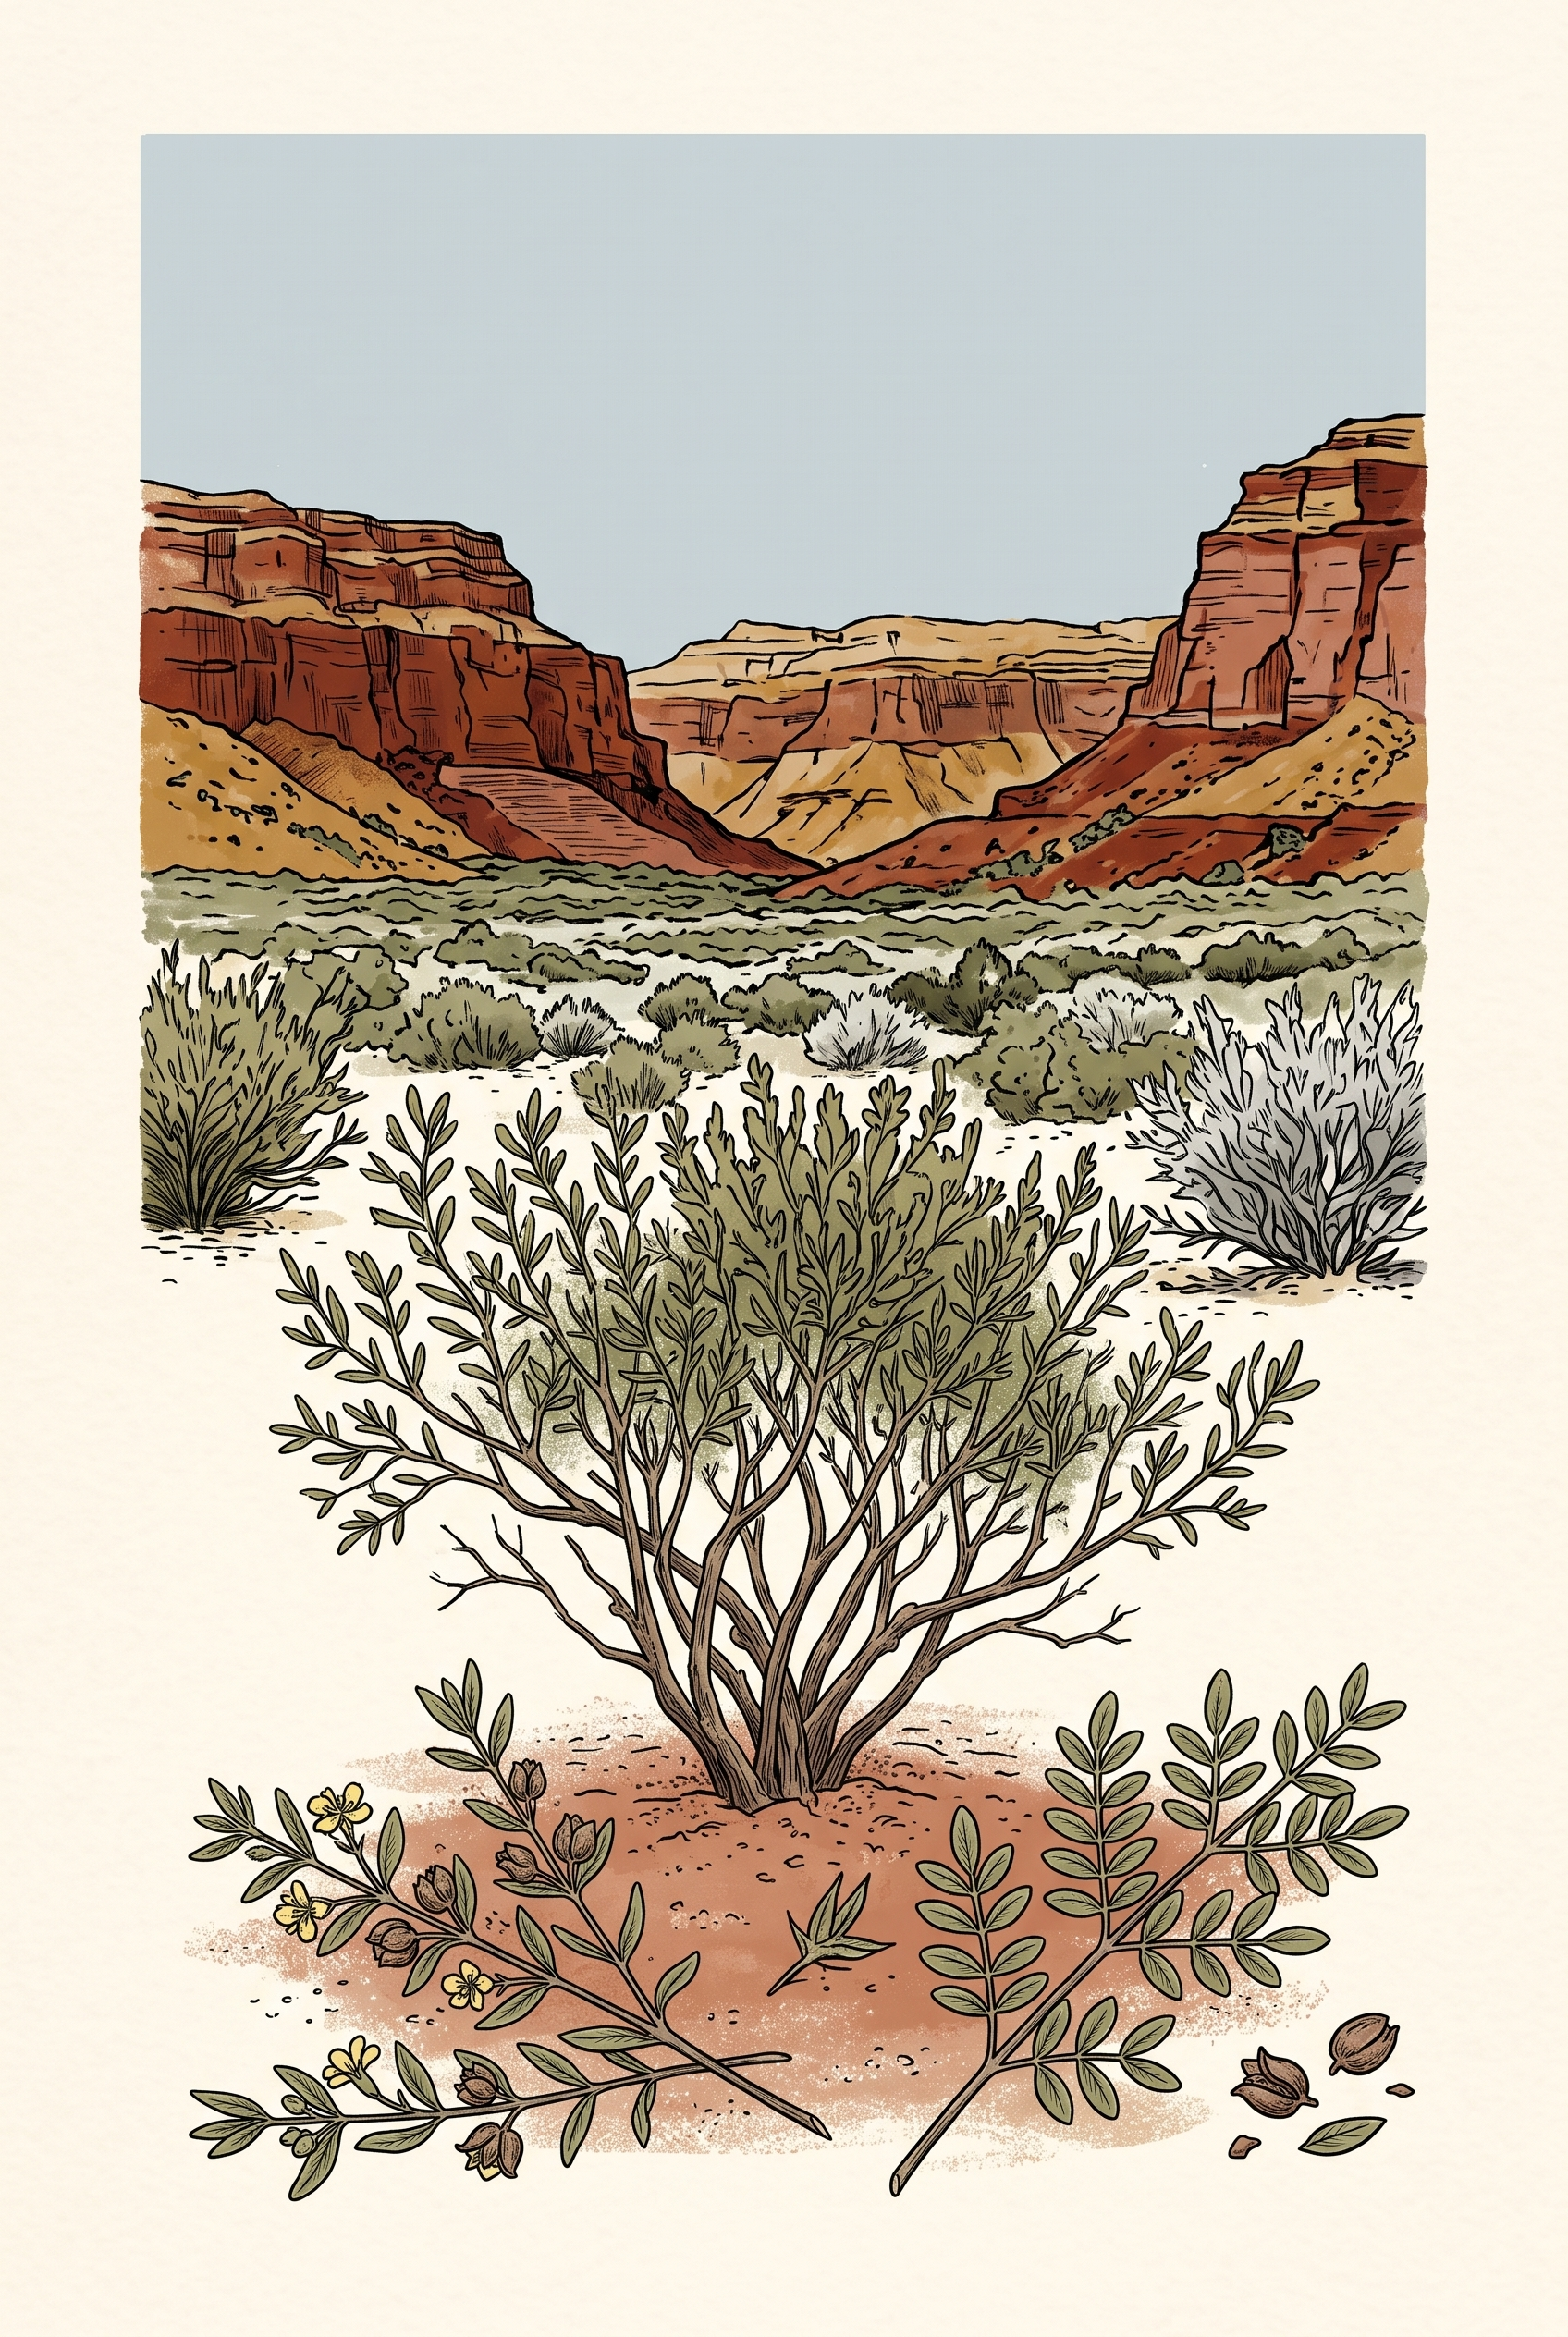
\includegraphics[width=\paperwidth,height=\paperheight]{img/23-contratapa.jpg}}}
\begin{tikzpicture}[remember picture, overlay]
  \fill[verdehuerta, opacity=0.64]
        (current page.north west) rectangle
        ([yshift=-8.2cm]current page.north east);
  \fill[verdehuerta, opacity=0.64, path fading=south]
        ([yshift=-8.2cm]current page.north west) rectangle
        ([yshift=-14.5cm]current page.north east);
  \node[anchor=north, inner sep=0pt] at ([yshift=-3.1cm]current page.north)
    {\begin{minipage}{0.76\paperwidth}
       \centering
       {\sffamily\fontsize{13}{17}\selectfont\color{crema} YUYOS DE LA QUEBRADA}\\[0.6em]
       {\color{ocre}\rule{3.4cm}{0.8pt}}\\[0.9em]
       {\itshape\small\color{crema}
        «Existe una idea antigua que dice que en un perímetro de un
        kilómetro a la redonda tenemos todo lo que necesitamos para
        sanarnos. Por eso considero al ser urbano huérfano de madre
        naturaleza.»}\\[1.2em]
       {\sffamily\fontsize{9.5}{12}\selectfont\color{crema}
        MARÍA EUGENIA ORELLANA}\\[0.8em]
       {\sffamily\fontsize{8}{11}\selectfont\color{crema}
        VALLES CALCHAQUÍES · SALTA}
     \end{minipage}};
\end{tikzpicture}
\null

\end{document}
